\chapter{Results and Conclusion}\label{ch:results-&-conclusion}
\section{Achievements and Results}
The main goals of this thesis have been met. Both of the extensions incorporate/integrate spatial data representations into OpenRefine and also integrate OpenStreetMap data into OpenRefine.
\subsection{OSM Extractor Results}
Integrating OpenStreetMap data into OpenRefine using the Overpass QL API:
\begin{itemize}
    \item Create an OpenRefine-friendly extension using OpenRefine\textquotesingle s extension architecture
    \item Use the Overpass API and Overpass QL queries to extract custom OpenStreetMap data
    \item Choose what tags to include in the OpenRefine project and also what type of geometry objects
    \item Assign the correct data types to the columns (text, number, date, column)
    \item Separate tags depending on their purpose and meaning. They can be \textit{Identifier, Main, Metadata or Other} tags
    \item Create user-friendly components throughout the whole extension
    \item Use OpenRefine\textquotesingle s core engine to create projects and log everything correctly
    \item Bundle, release and test the extension correctly and continuously using iterative \href{https://gitlab.com/labiangashi/osm-extractor/-/releases}{releases}
    \item Use CI/CD pipeline features to build the documentation and also build, test and \href{https://gitlab.com/labiangashi/osm-extractor/-/releases}{release new versions} of the extension
    \item Create \href{https://gitlab.com/labiangashi/osm-extractor/-/issues}{issues} and
    \href{https://gitlab.com/labiangashi/osm-extractor/-/milestones}{milestones} in the code repository host website to correctly describe and
    track the project\textquotesingle s process and features
\end{itemize}
\begin{figure}[H]
    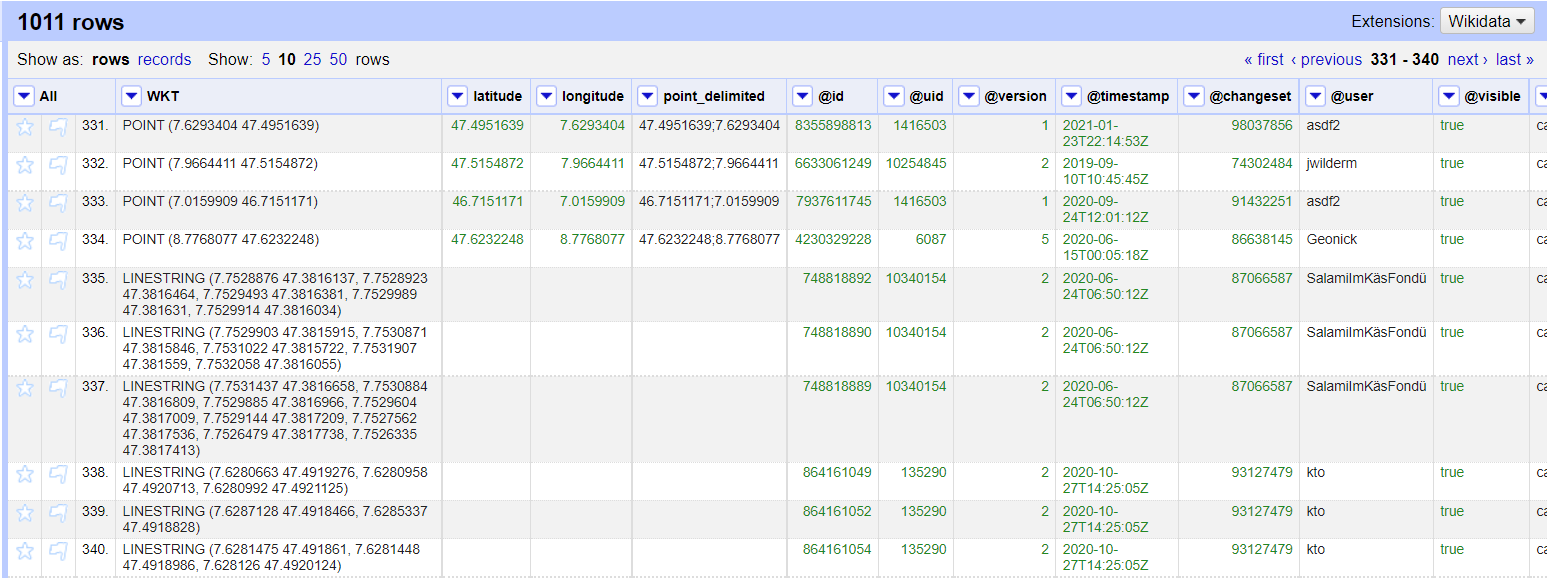
\includegraphics[width=\linewidth]{./Figures/Results/osm_extractor_results}
    \caption{OSM Extractor results in an OpenRefine project}
\end{figure}
\subsection{GeoJSON Export Results}
Exporting OpenRefine data to the GeoJSON (.geojson) format:
\begin{itemize}
    \item Create an OpenRefine-friendly extension using OpenRefine\textquotesingle s extension architecture
    \item Use the Well-Known Text spatial data representation format to represent geometry objects
    \item Create a user-friendly export dialog for exporting the data to GeoJSON
    \item Use OpenRefine\textquotesingle s core engine to export the data and log everything correctly
    \item Bundle, release and test the extension correctly and continuously using iterative \href{https://gitlab.com/labiangashi/geojson-export/-/releases}{releases}
    \item Use CI/CD pipeline features to build the documentation and also build, test and \href{https://gitlab.com/labiangashi/geojson-export/-/releases}{release new versions} of the extension
    \item Create \href{https://gitlab.com/labiangashi/geojson-export/-/issues}{issues} and
    \href{https://gitlab.com/labiangashi/geojson-export/-/milestones}{milestones} in the code repository host website to correctly describe and
    track the project\textquotesingle s process and features
\end{itemize}
\begin{minted}[tabsize=2, breaklines, linenos]{json}
{
  "type" : "FeatureCollection",
  "features" : [ {
    "type" : "Feature",
    "geometry" : {
      "type" : "Point",
      "coordinates" : [ 8.718769, 47.350209 ]
    },
    "properties" : {
      "amenity" : "drinking_water",
      "@id" : "8899069808"
    }
  }, {
    "type" : "Feature",
    "geometry" : {
      "type" : "LineString",
      "coordinates" : [ [ 7.7529493, 47.3816381 ], [ 7.7529443, 47.3816044 ] ]
    },
    "properties" : {
      "historic" : "castle_wall",
      "ruins" : "castle"
    }
  }, {
    "type" : "Feature",
    "geometry" : {
      "type" : "MultiPolygon",
      "coordinates" : [ [ [ [ 8.1404353, 46.1959036 ], [ 8.1404352, 46.195953 ], [ 8.1402542, 46.195952 ], [ 8.1401752, 46.1959494 ], [ 8.140174, 46.1958587 ], [ 8.140173, 46.1957775 ], [ 8.1404439, 46.1957792 ], [ 8.1404431, 46.1958362 ], [ 8.1403847, 46.1958358 ], [ 8.1403838, 46.1959033 ], [ 8.1404353, 46.1959036 ] ] ], [ [ [ 8.1404353, 46.1959036 ], [ 8.1404918, 46.195904 ], [ 8.1404928, 46.1958365 ], [ 8.1404731, 46.1958364 ], [ 8.1404431, 46.1958362 ], [ 8.1404353, 46.1958362 ], [ 8.1403847, 46.1958358 ], [ 8.1403838, 46.1959033 ], [ 8.1404353, 46.1959036 ] ] ] ]
    },
    "properties" : {
      "addr:housename" : "Stockalperturm",
      "historic" : "castle",
      "building:levels" : "5",
      "type" : "site",
      "addr:postcode" : "3907",
      "building" : "hotel",
      "addr:city" : "Gondo",
      "addr:housenumber" : "21",
      "material" : "stone",
      "castle_type" : "defensive",
      "name" : "Stockalperturm",
      "addr:street" : "Simplonstrasse",
      "wikidata" : "Q443634"
    }
  } ]
}
\end{minted}
Exported GeoJSON file containing geometries such as a \mintinline{bash}{Point}, a \mintinline{bash}{LineString}  and a \mintinline{bash}{MultiPolygon}.
\pagebreak
\section{Reflection and Conclusion}
Working with the OpenRefine application was a great experience for me. Their extension architecture is simple and efficient to understand and use.
Since OpenRefine is an open-source project, working with it also improved my ability to work in an open-source project
and know the approaches that are used by developers when developing open-source projects.\\
\newline
Although I have worked with OpenStreetMap before, in this thesis, close work was done with OpenStreetMap and the Overpass API. This allowed me to further
expand my knowledge on OpenStreetMap data and the Overpass API.\\
\newline
Working with geospatial data was also a great addition to my knowledge stack, since I had to work closely with geospatial data and open standards,
research needed to be done before making decisions on the extensions. This made me understand geospatial data and objects in a broader sense.\\
\newline
Finally, this thesis would have been much harder to implement if libraries like the ones that were used in this project didn\textquotesingle t exist. The work and effort
that would need to be put in implementing the extensions would expand and it would definitely question the feasibility of such a project.
\section{Outlook}
Contributions to the OpenRefine core project are also in the scope. One of the items discussed with the OpenRefine Dev Community is collaborating with them to continue implementing a feature that allow users to add descriptions and different custom metadata to their OpenRefine project\textquotesingle s columns. These works would go directly into the core OpenRefine project. The discussion can be viewed here: \href{https://groups.google.com/g/openrefine-dev/c/xWoWiAA6KhQ}{https://groups.google.com/g/openrefine-dev/c/xWoWiAA6KhQ}
\subsection{The OSM Extractor Extension}
The current version of the \textbf{OSM Extractor} extension successfully utilizes the Overpass API to integrate OpenStreetMap data into a new OpenRefine project. Future versions of OSM Extractor could save the Overpass query, similar to a saved database connection (connection string). Or it could allow synchronization to keep an OpenRefine
project up-to-date with OSM. The user would need a \textit{Sync} button on the OpenRefine project which would sync the current data with the latest updates/additions on the OpenStreetMap database. All the records would need to have their unique identifier stored, in order to know if they were updated or if new OpenStreetMap elements were added in OpenStreetMap. This feature would need a \textit{Sync} button somewhere on the project
where the user would click every now and then (depending on when they want to update the data) and all the new/updated data would be re-integrated into that same OpenRefine project.
\subsection{The GeoJSON Export Extension}
The \textbf{GeoJSON Export} extension is able to successfully export any type of \textit{Simple Feature} geometry object into GeoJSON, except the \mintinline{bash}{GeometryCollection} object.
Future versions of this extension could consider adding that type of Geometry as well into the supported GeoJSON geometry types.